\newpage

\chapter{Реализация}
\label{ch:chapter_2}

\section{Выбор технологий для реализации сетевой архитектуры}

\subsection{Выбор протокола промежуточного слоя}
\label{sec:choosing_middleware}
Проект HiveMind поддерживает мобильные устройства и настольные компьютеры (см.
пункт \ref{sec:project_summary}), имеющие различный способ подключения к
интернету. Как правило, настольные компьютеры имеют проводное соединение с сетью
интернет (Ethernet, ADSL), а мобильные устройства беспроводное (Wi-Fi, WiMax,
3G).

Проводное соединение имеет следующие особенности:
\begin{itemize}
\item широкий канал интернет соединения;
\item стабильность;
\item зависимость от расположения кабеля.
\end{itemize}

Особенности беспроводного соединения:
\begin{itemize}
\item узкий канал Интернет соединения;
\item высокая мобильность;
\item низкая стабильность;
\item задержки при передачи данных;
\item зачастую соединение расположено за NAT (отсутствует прямой доступ из сети
Интернет).
\end{itemize}

Пользователи как настольных, так и мобильных систем могут соединяться с сетью
Интернет через NAT, фаервол или прокси-сервер, не имея возможности установить
прямое соединение, примером является сетевая инфраструктура организации.

В соответствии с концепцией сетевого взаимодействия (см. пункт
\ref{sec:collaborative_mindmapping}), мы имеем клиент-серверную архитектуру. Для
удобства пользователей необходимо, чтобы клиентская и серверная части могли быть
созданы в любой момент времени и на любом устройстве. Взаимодействие должно
выглядеть следующим образом: пользователь создаёт сервер, другие участники
подсоединяются к нему и начинают редактирование. Каждое изменение, сделанное
участником, отправляется на сервер, который рассылает это изменение всем другим
участникам (см. рис. \ref{img:users_collaboration_example}).

\begin{figure}[!h]
  \centering
  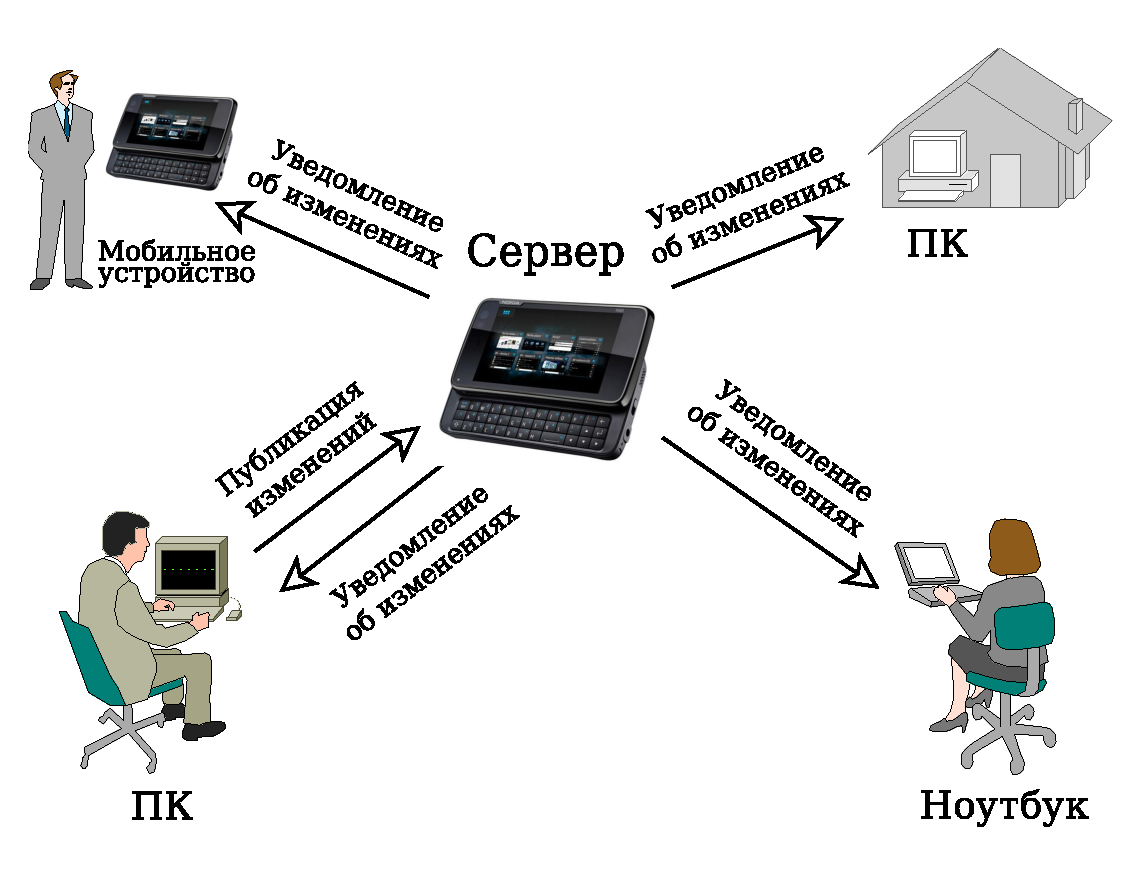
\includegraphics[width=\linewidth]{users_collaboration_example.pdf}
  \caption{Взаимодействие клиентов и сервера}
  \label{img:users_collaboration_example}
\end{figure} 

Подводя итог всему вышеперечисленному, был сформирован список требований к
выбираемой технологии промежуточного слоя:
\begin{itemize}
\item взаимодействие основанное на клиент-серверной модели;
\item не должно быть сложностей в создании сервера;
\item сервер должен иметь возможность уведомления всех участников
взаимодействия;
\item технология должна хорошо работать в условиях медленного, ненадежного
соединения с сетью Интернет, расположенного за NAT, прокси-сервером или
фаерволом.
\end{itemize}

Протокол XMPP c расширением публикации/подписки полностью удовлетворяет
вышеназванным требованиям и позволяет избежать почти все сложности, связанные с
реализацией клиент-серверной архитектуры, 

\subsection{Преимущества протокола XMPP}
XMPP (Extensible Messaging and Presence Protocol) "--- расширяемый протокол для
обмена сообщениями, в режиме близком к режиму реального времени. Протокол XMPP
может быть рассмотрен на нескольких уровнях абстракции. На нижнем уровне
абстракции, существует клиентское приложение, использующее протокол XMPP,
которое подключается к серверу и обменивается с ним сообщениями. Соединение с
сервером может быть установлено несколькими способами, даже поверх протокола
HTTP. На высоком уровне абстракции, клиент получает доступ ко всей XMPP сети,
где каждый её узел имеет уникальный идентификатор, называемый JID (Jabber
Identificator). Преимуществом протокола XMPP является то, что пересылка
сообщений между узлами сети не требует дополнительных усилий. Клиент создаёт
сообщение, адресованное другому клиенту и посылает его на сервер, который
отвечает за все операции, связанные с доставкой данного сообщения.

Большое преимущество протокола XMPP "--- расширяемость. Он может быть расширен с
помощью расширяющих протоколов (XEP). XMPP является открытым протоколом и каждый
желающий может создать высокоуровневый протокол на его основе. Организация XMPP
Standards Foundation отвечает за процесс создания и поддержки данных протоколов.
Одно из подобных расширений называется XEP-0060 Publish-Subscribe
\cite{xep-0060}. Оно отвечает за то, как реализовывать сервис
публикации/подписки поверх протокола XMPP. Любой участник XMPP сети имеет
возможность создать сервис публикации/подписки.

XMPP был создан как протокол мгновенного обмена сообщениями, использующий XML
для формирования сообщений. XML создаёт большой объём служебной информации, что
может потребовать широкой полосы Интернет соединения. В XMPP сети, сообщения
между клиентом и сервером могут быть сжаты с использованием XEP-0138 (Stream
Compression). Таким образом, протокол XMPP имеет механизм, позволяющий
использовать его в сетях с малой полосой пропускания.

В настоящее время существует множество общедоступных XMPP серверов
поддерживающих общение в чате. Участие в подобных чатах доступно с мобильных
устройств и не требует широкополосного доступа в Интернет. С технической точки
зрения, совместное редактирование диаграмм очень похоже на участие в чате из
чего следует, что объём трафика не будет сильно отличаться. Исключением является
устройство, являющееся сервером. Данному устройству будет необходим более
широкий канал до сети Интернет для взаимодействия со многими клиентами.

\subsection{Выбор библиотеки для работы с протоколом XMPP}
Следующей задачей является выбор библиотеки языка Python, поддерживающей работу
с протоколом XMPP. На сайте XMPP Foundation \cite{xmpp} есть список
из восьми библиотек поддерживающих XMPP. Некоторые библиотеки более не
поддерживаются (jabber.py), некоторые требуют использования более новых (2.6,
3.x) версий языка Python, недоступных под платформой Maemo (pyxmpp), другие же
являются исследовательскими проектами и не предназначены для повсеместного
использования (SleekXMPP). Twisted "--- единственный инструмент для работы с
протоколом XMPP, доступный в репозитории Maemo.

Twisted "--- событийно-ориентированный сетевой фреймворк, поддерживающий
множество протоколов таких как: TCP, UDP, SSL/TLS, HTTP, XMPP, NNTP, IMAP, SSH,
IRC, FTP и множество других \cite{twisted}. Twisted не имеет встроенной
поддержки XEP-0060, но существует внешняя библиотека Wokkel \cite{wokkel},
поддерживающая данное расширение. Данная библиотека отсутствует в репозитории
Maemo. Для того, чтобы иметь возможность её использовать, было принято решение о
создании и поддержки пакета для платформы Maemo.

\section{Архитектура сетевой подсистемы}
\subsection{Расширение XMPP с поддержкой публикации/подписки}
Расширение XEP-0060 использует шаблон проектирования <<публикация/подписка
(publish-subscribe)>>, являющийся более общим относительно шаблона <<наблюдатель
(observer)>>. Данный шаблон состоит в следующем: объект подписывается на
обновления от другого объекта и становится его подписчиком. После того, как
подписчик публикует информацию, уведомление о данном событии (с опубликованной
информацией или без) пересылается всем подписчикам. В общем случае,
взаимодействие между подписчиками контролируется сервером, который получает
запрос на публикацию и производит рассылку уведомлений всем подписчикам.

Сервер может поддерживать подписку на различные сущности. В терминах расширения
XEP-0060, данные сущности называются узлами (nodes). Каждый подобный узел имеет
собственный список подписчиков. Узлы также могут хранить историю всех
уведомлений и обеспечивать другие сервисы определённые стандартом. Данные
получаемые сервером и пересылаемые на него называются элементом (item).
Описанная система организации данных может быть ассоциирована с организацией
файловой системы, где узлы представляют директории, а элементы соотносятся как
файлы.

В терминах расширения XMPP публикации/подписки, процесс
взаимодействия может быть представлен следующим образом. Пользователь создаёт сервер с единственным
узлом для обмена и хранения сообщений. Другие участники подписываются на
обновления от созданного узла. Когда один из публикующих делает изменения, они
пересылаются на сервер, который уведомляет всех подписчиков о произошедшем
событии. Данные пересылаются, используя возможности элемента содержать в себе
полезную нагрузку. Учитывая характер процесса взаимодействия между сервером и
подписчикам, была начата разработка сетевой архитектуры приложения.

\subsection{Распространение изменений}
\label{sec:changeset_propagation}
Приложение HiveMind, как и любой хороший редактор, имеет возможности отмены и
повтора ранее отмененных действий. Данная функциональность реализована на основе
QUndoStack, который хранит всю историю выполненных команд. Каждое изменение на
диаграмме связей атомарно. Когда пользователь совершает изменение создаётся
QUndoCommand. В QUndoCommand хранится информация для выполнения команды и для её
отката. Таким образом, использование QUndoStack позволяет двигаться по всей
истории изменений. Для каждого типа данных команд были созданы функции
сериализации и десериализации в XML. Изменения сделанные на карте отправляются
на сервис в виде XML сериализованных сообщений и не сохраняются в стеке команд.
Команды добавляются в стек только если они пришли как уведомления от сервиса,
поэтому подписчик должен ждать ответа от сервера для того чтобы увидеть
выполненные изменения (см рис. ~\ref{img:changeset_propagation}).

\begin{figure}
  \centering
  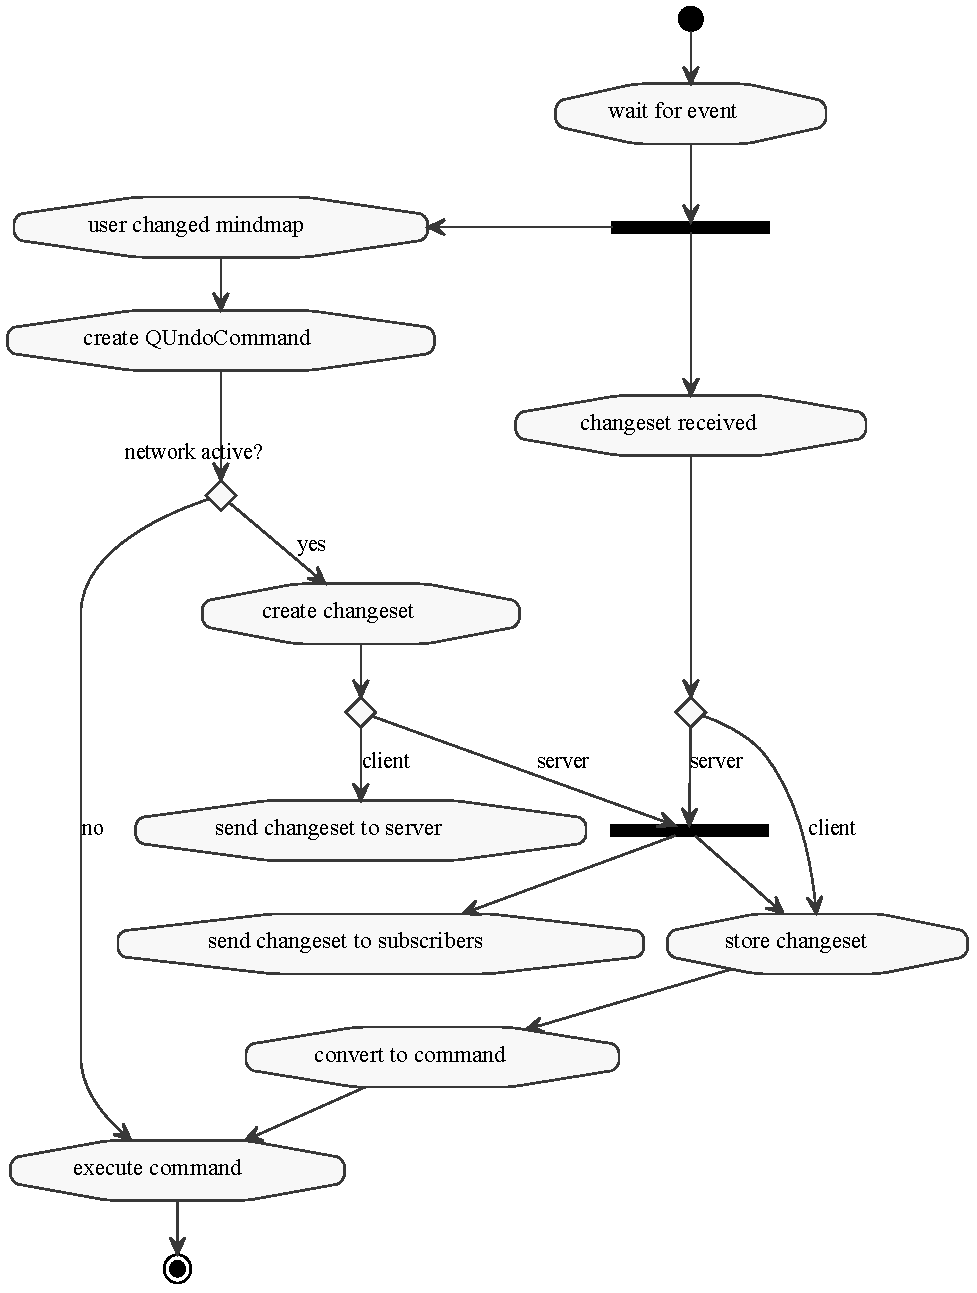
\includegraphics[width=\linewidth]{changeset-propagation.pdf}
  \caption{Диаграмма распространения изменений}
  \label{img:changeset_propagation}
\end{figure}

Для того чтобы управлять асинхронным взаимодействием был реализован класс
NetworkController. Все команды поступают в сетевой контроллер. Если сетевое
взаимодействие неактивно, команда добавляется в стек команд. В противном
случае, данная команда будет сериализована и отправлена на сервис. Уведомления
пришедшие от сервиса десериализуются в команды, добавляются в стек команд и
выполняются.

Данные команды содержат в себе информацию лишь об изменившейся части диаграммы.
Подобное условие необходимо для того, чтобы уменьшить объём пересылаемых данных,
который в противном случае будет чрезмерно большим. Необходимо чтобы все
участники имели одинаковые копии диаграмм, иначе команда, являющаяся корректной
с точки зрения одного участника, не будет являться таковой для другого. Поэтому
встаёт вопрос о распространении исходной диаграммы и её синхронизации между
всеми участниками в процессе взаимодействия.

Проблема распространения диаграммы была решена следующим образом: первый элемент
в узле должен содержать в себе сериализованную диаграмму связей. Все остальные
элементы содержат в себе сериализованные команды изменений. В момент, когда
человек становится подписчиком, ему пересылаются все элементы содержащиеся в
узле, включая диаграмму и совершенные ранее изменения.

Синхронизация диаграммы связей между всеми участниками представляет более
сложную проблему. Фактически речь идёт о сохранение целостности диаграммы связей
на сервере, то есть о контроле поступающих изменений. При поступлении
некорректного изменения, сервер должен его отбросить или провести слияние, если
возможно. К примеру, из-за задержек в соединении, пользователь может изменить
узел, который к этому времени уже был удалён одним из участников. В таком случае
сервер отсылает пользователю уведомление об ошибке и отбрасывает некорректное
изменение.

Подписчик может запросить все данные или часть данных, хранящихся в узле, в
любой момент времени. Данная возможность используется для синхронизации
локальной копии диаграммы с копией на сервере. К примеру, если изменение было
отброшено сервером, то подписчик производит синхронизацию своей диаграммы с её
версией на сервере. Сервер не нуждается в дополнительных способах синхронизации
диаграммы, поскольку все изменения локальны и всегда являются актуальными и
корректными.

\section{Реализация сетевой подсистемы}
Сетевая подсистема приложения была реализована поверх фреймворка Twisted и
библиотеки Wokkel. Wokkel является надстройкой над Twisted, добавляющей
фреймворку дополнительную функциональность. В частности Wokkel предоставляет
средства для более удобной реализации расширений XMPP (XEP) и имеет поддержку
следующих: Service Discovery (XEP-0030), Publish-Subscribe (XEP-0060).
Реализация расширения публикации/подписки в Wokkel не содержит бизнес-логики.
Это значит, что он отвечает за приём, генерацию и отправку сообщений в
соответствии со спецификацией XEP-0060. Wokkel реагирует на события, относящиеся
к публикации/подписке, делает разбор пришедших сообщений и вызывает
соответствующие обработчики.

Расширение публикации/подписки является одним из самых больших и сложных
стандартов XMPP. Реализация необходимого функционала, корректная с точки зрения
стандарта, могла занять большое количество времени. Поэтому было принято решение
использовать библиотеку Idavoll. Данная библиотека реализована на базе Wokkel и
реализует функциональность XEP-0060 необходимую для приложения, такую как:
<<Подписка>>, <<Публикация>>, <<Создание узлов>>, <<Хранилище элементов>>.
Библиотека Idavoll имеет хорошую архитектуру, позволяющую добавлять реализацию
новой функциональности, определенной стандартом расширения публикации/подписки.
Idavoll имеет множество классов необходимых для реализации стандарта XEP-0060
(см. рис. ~\ref{img:network_classes}).

Класс Node является абстрактным классом и представляют собой узел в терминах
XEP-0060. Существуют два типа узлов: LeafNode и CollectionNode. LeafNode может
содержать только элементы, когда как CollectionNode может содержать лишь другие
узлы. LeafNode хранит элементы в виде простого списка, но это не является
подходящим решением для приложения HiveMind. Как было сказано в главе
~\ref{sec:changeset_propagation}, необходимо проверять приходящие изменения на
корректность. Для этого был создан класс Changeset, хранящий в себе информацию о
самом изменении, его типе, времени создания и авторе данного изменения. Также
создан специальный класс-контейнер СhangesetStack, хранящий экземпляры класса
Changeset и отвечающий за корректность и согласованность изменений находящихся в
нём. HivemindNode унаследован от LeafNode и в отличие от него хранит изменения в
ChangesetStack (исходный код в приложении ~\ref{ap:HivemindNode}).

\begin{figure}
  \centering
  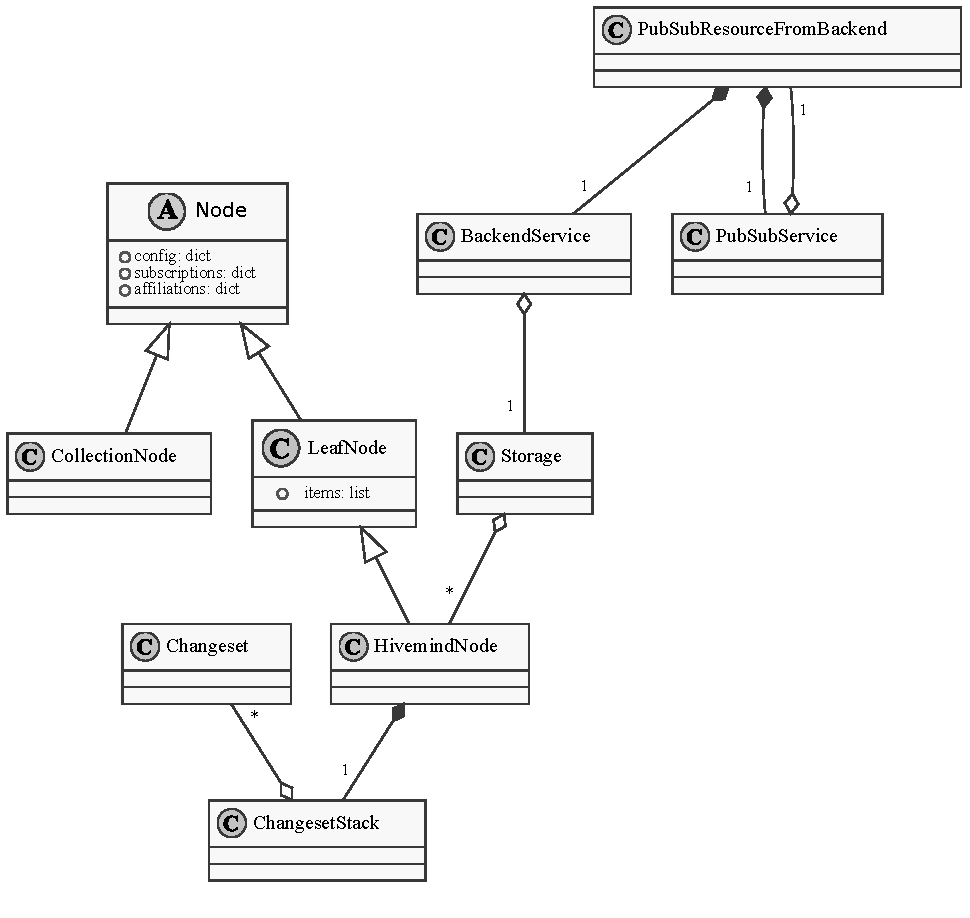
\includegraphics[width=\linewidth]{idavoll-classes.pdf}
  \caption{Диаграмма сетевых классов}
  \label{img:network_classes}
\end{figure}

BackendService содержит реализацию бизнес-логики XEP-0060. В нем содержится
логика для работы с подписчиками, проверка прав доступа и т.д. Он связан
отношением композиции с классом Storage, отвечающим за управление узлами
(создание, удаление, конфигурирование). Класс HivemindNode, создаётся классом
Storage и содержит в себе методы для добавления данных, изменения конфигурации
узла, списка подписчиков и их ролей. PubSubService является классом библиотеки
Wokkel, отвечающим за разбор пришедших сообщений и вызов соответствующих
обработчиков. Если он содержит в себе экземпляр класса
PubSubResourceFromBackend, то помимо вызова своих обработчиков, осуществляется
передача уже разобранных сообщений в подходящие методы класса
PubSubResourceFromBackend. Этот класс является дополнительным
уровнем абстракции, что позволяет делать архитектуру более гибкой.
PubSubResourceFromBackend обязательно содержит экземпляр класса BackendService,
которому он делегирует реализацию бизнес-логики.

На стороне клиента взаимодействие управляется классом HivemindClient (исходный
код в приложении ~\ref{ap:HivemindClient}). После установления соединения с
сервером XMPP, он запрашивает все элементы у сервиса HiveMind, отвечает за
обработку приходящих элементов и уведомляет NetworkController о поступивших
изменениях.

Мобильные устройства зачастую имеют нестабильное соединение с сетью Интернет,
поэтому приложение должно иметь механизм, позволяющий обнаружить, что соединение
потеряно и уведомить об этом пользователя. Механизм проверки осуществляется
посредством XMPP Ping (XEP-0199) \cite{xep-0199}. Класс Pinger ответственен за
отсылку пинг сообщений и приём ответов (исходный код в приложении
~\ref{ap:Pinger}). Проверка осуществляется следующим образом: данный класс
непрерывно отсылает пинг сообщения на XMPP сервер, к которому подключен
пользователь, если достигнуто определенное количество пинг сообщений, оставшихся
без ответа, то соединение рассматривается как потерянное. Pinger уведомляет
NetworkController о состоянии соединения с XMPP сервером, а также со всеми
подписчиками. Пользователь может увидеть статус соединения с подписчиками в
диалоге редактирования прав доступа(см. рис. ~\ref{img:permissions_dialog})

Похожий механизм используется для проверки статуса подписчиков. Каждый подписчик
имеет свой экземпляр класса Pinger, который отвечает за отсылку пинг сообщений
именно ему. На клиентской стороне реализован обработчик, который отвечает на
приходящие пинг сообщения от сервера приложения. Подписчиков может быть очень
много, поэтому был создан класс PingManager, отвечающий за управление
экземплярами класса Pinger (см. рис. ~\ref{img:ping_manager}). Он создаёт и
удаляет экземпляры класса Pinger, а также запускает или останавливает отправку
пинг сообщений до адресата (исходный код в приложении ~\ref{ap:PingManager}).

\begin{figure}
  \centering
  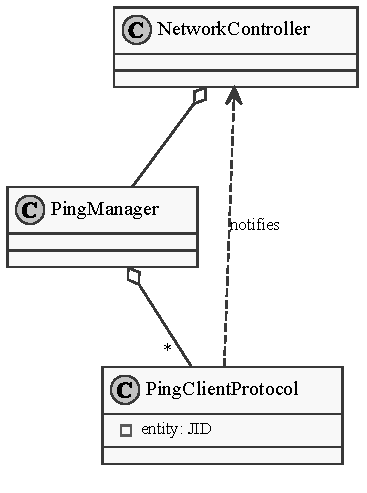
\includegraphics[scale=1.2]{ping-manager.pdf}
  \caption{Диаграмма классов, отвечающих за проверку состояния соединений}
  \label{img:ping_manager}
\end{figure}


\section{Система контроля доступа}
По умолчанию, все участники совместной работы имеют одинаковый доступ к
редактированию диаграммы связей. Такое поведение является подходящим для
случаев, когда необходимо создать множество идей или найти решение сложной
проблемы. Но существуют сценарии совместной работы, описанные в пункте ~\ref
{sec:collaborative_mindmapping}, при которых необходимо ограничить права доступа
некоторых пользователей. Для того, чтобы была возможность взаимодействия по
подобным сценариям, в HiveMind была реализована система контроля доступа.

Стандарт XEP-0060 заложена функциональность называемая моделью доступа (access
model), которая может быть сопоставлена с системой аутентификации. Пользователь,
открывающий доступ к диаграмме, может установить уровень доверия для новых
участников. Это значит, что пользователь может ограничить круг лиц, имеющих
право на присоединение к совместной работе. Было реализовано четыре модели
доступа:
\begin{itemize}
\item <<открытая (open)>> --- поведение по умолчанию,  любой может
присоединиться;
\item <<контакт лист (roster)>> --- только лица, находящиеся в контакт листе
владельца сервера имеют право на участие;
\item <<интерактивная (authorize)>> --- владелец может выбирать тех, кто имеет
право на участие в совместной работе. Когда очередной человек подключается к
диаграмме, владелец получает запрос на присоединение;
\item <<белый список (whitelist)>> --- новый участник может присоединиться, лишь
в том случае, если он находится в белом списке владельца сервера.
\end{itemize}

Следующая часть системы контроля доступа также заложена в стандарт XEP-0060 и
называется affiliations. Данная функциональность отвечает за авторизацию
пользователей. Каждый участник, присоединившийся к диаграмме, имеет свою роль,
определяющую набор допустимых действий. Было реализовано четыре роли:
\begin{itemize}
\item <<изгнанник (outcast)>> --- не имеет права присоединяться и участвовать в
совместной работе;
\item <<участник (member)>> --- имеет право только получать данные;
\item <<издатель (publisher)>> --- имеет право получать и публиковать данные;
\item <<владелец (owner)>> ---  имеет права издателя и может дополнительно
конфигурировать все аспекты сетевого взаимодействия.
\end{itemize}
Владелец сервера может в любой момент изменить роль человека, используя диалог
управления правами доступа (см. рис. ~\ref{img:permissions_dialog}).

\begin{figure}
  \centering
  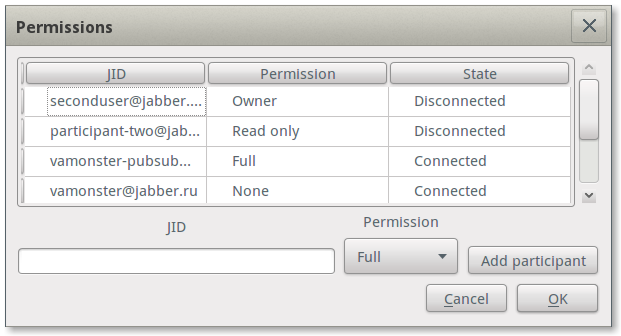
\includegraphics[width=0.8\linewidth]{permissions_dialog.png}
  \caption{Диалог управления правами доступа}
  \label{img:permissions_dialog}
\end{figure}

XEP-0060 предоставляет возможность сделать систему контроля доступа еще более
гибкой. В некоторых случаях, может возникнуть необходимость временно позволить
всем участникам редактировать диаграмму. Для этого можно изменить роли всех
участников на издателя, что в случае большого количества участников является
утомительным и долгим занятием. Выходом из данной ситуации является реализация
функциональности называемой моделью публикации (publish model), определенной
стандартом XEP-0060. Данный механизм определяет, кто имеет право вносить
изменения на диаграмму связей. Было реализовано две модели публикации. Первый
тип модели позволяет вносит изменения участникам, имеющим роль издателя или
владельца. Во втором случае, все присоединившиеся участники имеют право на
внесение изменений.

Реализация системы контроля доступа позволила значительно увеличить количество
сценариев совместного взаимодействия. Данная система может быть улучшена, чтобы
увеличить количество областей применения приложения. Одной из подобных областей
является проведение презентаций, а точнее взаимодействие докладчика и
слушателей. В пункте ~\ref{sec:collaborative_mindmapping} был представлен
сценарий проведения презентации. Данный сценарий может расширен следующим
образом: позволить слушателям добавлять свои вопросы и пожелания на диаграмму
докладчика. В таком случае, необходимо, чтобы слушатели не могли изменять узлы
созданные докладчиком или другими слушателями, за что и будет отвечать
усовершенствованная система контроля доступа.
